\documentclass[twoside,twocolumn,10pt]{jsarticle}
\usepackage{latexsym}        % 数学記号を増やすためのパッケージ
\usepackage{amssymb,amsmath} % 複雑な数式を書くためのパッケージ
\usepackage[dvipdfmx]{graphicx} % グラフィクスを使うためのパッケージ
\usepackage{enumerate}       % enumerate環境を高機能にするためのパッケージ
\usepackage{stabst}         % 理工学部の予稿用スタイル
%\english %英語で論文を書く場合に宣言する. jasrticle の代わりに article を使用すること. 
\usepackage{listings,jvlisting} %日本語のコメントアウトをする場合
%ここからソースコードの表示に関する設定
\usepackage[hyphens]{url}
\usepackage[dvipdfmx]{hyperref}
\usepackage{autobreak}

\renewcommand{\lstlistingname}{ソースコード}
\renewcommand{\lstlistlistingname}{ソースコード一覧}

\Urlmuskip=0mu plus 1mu\relax

\lstset{
  basicstyle={\ttfamily},
  identifierstyle={\small},
  commentstyle={\smallitshape},
  keywordstyle={\small\bfseries},
  ndkeywordstyle={\small},
  stringstyle={\small\ttfamily},
  frame={tb},
  breaklines=true,
  columns=[l]{fullflexible},
  numbers=left,
  xrightmargin=0zw,
  xleftmargin=3zw,
  numberstyle={\scriptsize},
  stepnumber=1,
  numbersep=1zw,
  lineskip=-0.5ex
}
%ここまでソースコードの表示に関する設定
\def\labelenumi{(\theenumi)}

\title{誤り指摘に基づくペアプログラミング指示評価システムの提案}

% \subtitle{—要旨の場合—} % 副題がない場合はこの行をコメントアウトする.
                        % 副題を囲む横棒は全角ダッシュ文字を使う.
\author{2022TS008 藤井洸 \ \ 2022TS037 松本輝央 \ \ 2022TS069 高橋侑暉}
\professor{指導教員:吉田敦}

\begin{document}
\maketitle

\section{はじめに}\label{sec:はじめに}
近年,ソフトウェア開発において,ペアプログラミングは開発効率やコードの品質向上に寄与する手法として注目を集めている\cite{begel2008pair}.ペアプログラミングでは,2人の開発者が「ドライバ」と「ナビゲータ」という役割に分かれ,協力して1つのプログラムを作成する.ドライバが実際にコードを書く一方で,ナビゲータは設計や戦略の観点から指示を出す.このような協働作業により,開発者はドライバとして実践を積むことで,短期間で技術や知識を修得し,開発能力を高められる.

一方で,ナビゲータの役割は,ある程度の技術的能力があれば担えるが,ドライバに適切な指示を出すには,経験とスキルが必要である.もし指示が不適切であれば,仕様を満たさないプログラムが作成され,むしろ開発効率が低下する恐れがある.ナビゲータに求められる能力のひとつに,自身の暗黙的な知識を明確な言葉で伝える「指示の言語化」があるが,これは必ずしも容易ではなく,訓練を必要とする.

ナビゲータの指示力を育成するためには,現実のペアプログラミングと同様に,ドライバの作業を観察し,そこに含まれる誤りを見抜き,適切な修正指示を出すという実践的な経験を積むことが不可欠である.しかし,学習者同士でペアを組んで訓練を行う場合,互いの理解度や経験に差があるために,誤りが正しく指摘されなかったり,不適切な指示がそのまま受け入れられたりする可能性が高い.その結果,学習効果が安定せず,評価の標準化も困難となる.

現在,生成AIの急速な進展により,プログラム生成を生成AIに任せることで,ドライバの役割をAIが担うことが可能になりつつある\cite{Surveyre96:online}.このような環境では,ユーザはナビゲータの役割を自然に体験できるが,実際に出した指示が適切であったかを評価する機能は備わっていない.そのため,ナビゲータとしての指示力を体系的に鍛えるには不十分である.

本研究の目的は,ナビゲータの指示の適切さを評価し,フィードバックを行うペアプログラミング練習システムを提案する.本システムでは,ナビゲータが行う主要な指示のうち,「誤りの指摘」に注目し,その適切さを評価する.生成AIがドライバとして提示するプログラムには意図的に誤りが含まれており,ナビゲータはそれらの誤りを指摘・修正する指示を与える.システムは,ナビゲータの指摘がすべての誤りを網羅しているか,また指示が正しく修正を導く内容であるかを評価し,指摘漏れや誤った修正をフィードバックすることで,指示能力の向上を支援する.

本システムの実現には次の課題がある.まず,ドライバが生成するプログラムにどのような誤りを,どのように混入させるかという点である.本研究では,ドライバが犯しうる誤りのパターンを分類・整理し,それぞれに対する混入方法を検討する.また,ナビゲータの修正指示の適切さをどのように評価するかも重要な課題である.本研究では,関数の仕様と正解例のプログラムを前提とし,ナビゲータの指示に基づいて生成AIが修正したプログラムと正解例とを比較することで,指示の妥当性を評価する.ただし,生成AIは必ずしも正解例と同一のコードを出力するとは限らないため,その比較方法についても工夫が必要である.

本システムの課題は,ナビゲータの修正指示の適切さをどのように評価するかである.本システムでは,関数の仕様と正解例のプログラムを前提とし,ナビゲータの指示に基づいて生成AIが修正したプログラムと正解例とを比較することで,指示の妥当性を評価する.ただし,生成AIは必ずしも正解例と同一のコードを出力するとは限らないため,その比較方法についても工夫が必要である.

\section{関連研究}\label{sec:関連研究}

近年,生成AIの進化により,学習者が一人でも擬似的なペアプログラミングを実践できる自己学習手法が注目されている.なかでも,AIを仮想のペアと見立て,学習者と交互に「ドライバ(コードを書く)」と「ナビゲータ(指示を出す)」の役割を担う形式は,協働的思考を再現できる点で有効なアプローチとされる.

既存研究では,AIとの対話を通じて設計や修正の指示を行う演習を通じ,プログラミングに必要な多角的思考力や論理的説明力を養うことが目的とされている.また,学習者は演習後に気づきや工夫を振り返りシートに記録することで,内省的な学びを深めていた\cite{原田紗希2024生成}.

本研究はこれらのアプローチを踏まえつつ,特にナビゲーターとしての「指示力」の育成に焦点を当て,AIが提示する誤りを含むコードに対して,学習者が適切に指示・修正を行う課題を設計している.さらに,指示内容の「網羅性」や「正確性」を自動で評価・フィードバックする機構を備えることで,指導力の客観的な測定と継続的な改善を可能とする.

従来の研究が「一人でも協働的に学べる環境」の提供に主眼を置いていたのに対し,本研究は「誤りを見抜き,適切に指示する力」の育成と評価に特化している点において,新たな意義を有するといえる.

\section{提案の内容}\label{sec:提案の内容}
システムの設計にあたっては,教育的効果や運用可能性を考慮し,明確な学習プロセスを設定する必要がある.以下ではまず,前提となる学習プロセスを説明し,続いて,提案内容であるナビゲータの指示の評価方法を説明する.

\subsection{前提とする学習プロセス}
本システムは,以下の5つの学習手順を前提とする.

\begin{description}
    \item[手順1] 教員による問題提示
        \begin{itemize}
            \item 教員は,プログラミングの問題と,作成するべき関数の引数と返り値を渡す.
            \item 例:「ユーザーがタスクを管理できるtodoリストを作成せよ」など
        \end{itemize}
    \item[手順2] 学習者によるアルゴリズム設計
        \begin{itemize}
            \item 学習者は問題を読んで,関数のアルゴリズムや処理手順を考える.
            \item ここではまだソースコードは書かない.
        \end{itemize}
    \item[手順3] ドライバAIによるコード生成(意図的な誤りを含む)
        \begin{itemize}
            \item 学習者が設計したアルゴリズムをもとに,ドライバAIがプログラムコードを生成する.
            \item このとき,AIはわざと小さな誤り(例:変数名の不一致,境界条件の不備,型の取り違えなど)を,関数毎に混入させる.
        \end{itemize}
    \item[手順4] 学習者による誤りの指摘と修正指示
        \begin{itemize}
            \item 学習者はナビゲータとして,生成されたコードを読み,誤りを特定してAIに修正を指示する.
            \item ドライバAIは学習者の指示に従って修正コードを再生成する.
            \item その際,評価システムを利用して,学習者の指示を評価する.
            \item 誤りがなくなるまでこの対話を繰り返す.
        \end{itemize}
    \item[手順5] 完成したプログラムの提出
        \begin{itemize}
            \item 学習者は,教員に完成したプログラムを提出する.
        \end{itemize}
\end{description}

この中で,提案システムが主に関与するのは「手順3」と「手順4」である.手順3 では,学習者が設計したロジックに対して,ドライバ役の生成AIがプログラムコードを出力する.このAIが提示するコードには,あらかじめ設計された誤りが意図的に含まれている.手順4において,学習者はナビゲータとして,提示されたコードを確認し,誤りを見つけて修正するようAIに指示を出す.その指示の内容をシステムが解析・評価し,学習者にフィードバックを行うことで,指示能力の向上を図る.

\subsection{提案システムの概要}
本研究が提案するシステムは,学習者がナビゲータとしての役割を実践的に学習できる環境を提供することを目的とする.システムは,生成AIをドライバ役として利用し,あらかじめ提示されたコードに対して学習者が修正指示を与えることで,ナビゲータとして必要な「誤り発見能力」と「修正指示能力」を繰り返し訓練できる.

システムの基本構成は,(1)ナビゲータ指示入力モジュール,(2)指示評価モジュールの2つからなる.ナビゲータ指示入力モジュールでは,学習者がコードの誤りを発見し,自然言語で修正方針をドライバに伝える.その後,指示評価モジュールが入力内容を解析し,修正指示の正確さや具体性を評価する.評価結果は学習者にフィードバックされ,必要に応じて修正を繰り返すことで,ナビゲータとしての指示力を段階的に向上させることができる.

\begin{figure}[h]
  \centering
  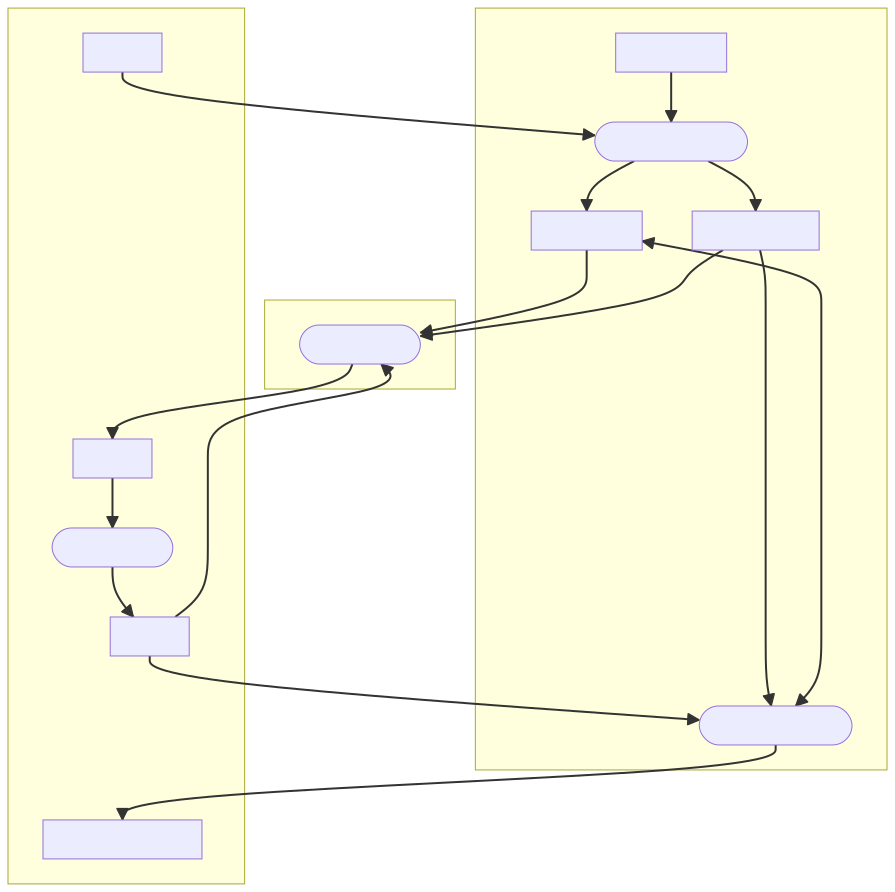
\includegraphics[width=1\linewidth]{module.pdf}
  \caption{システムのモジュール構造図}
\end{figure}

\subsection{ナビゲータの指示の評価方法}
ナビゲータがAIに与える指示の適切さを評価するためには,以下の2点を満たしているかを基準とする.
\begin{enumerate}
    \item 指摘の網羅性:ドライバAIが提示したコードに含まれるすべての誤りに対して,ナビゲータが漏れなく指摘できているか.
    \item 修正内容の正確性:各誤りに対して,修正方針や内容が正確であり,仕様を満たすように導けているか.
\end{enumerate}

\subsection {指示評価方法の比較}
指示評価モジュールにおける評価方法を決定するにあたり,以下の4つの方法を検討する.

\subsubsection*{方法1:テストケース実行による評価}
修正指示に基づいて生成されたコードをテストケースで実行し,正しい出力が得られるかを判定する方法である.利点として,評価が客観的で自動化しやすい点が挙げられる.  
しかし,テストケースで正しい出力が得られても,学習者の指示が誤りを十分に網羅しているかや,修正方針が適切であるかは測定できない.すなわち,「出力が正しい=適切な指示を行った」とは限らない.  
また,生成AIによる評価とテストケースを組み合わせたハイブリッド方式も考えられるが,本研究の目的は「指示の内容そのものの妥当性を評価し,ナビゲータとしての指示力を育成すること」にある.テストケース方式はあくまで結果(コードの動作)しか判定できず,指示内容の良否を直接扱うことができないため,ハイブリッド化しても本質的な課題は残る.  
したがって,本研究ではテストケース方式を主たる評価方法として採用しない.

\subsubsection*{方法2:構文木(AST)やコード構造の比較}
修正後のコードと正解コードを抽象構文木(AST)レベルで比較する方法である.文字列比較の場合,変数名の違いやインデントの違いといった表面的な差異も「不一致」と判定されるが,AST比較ではコードの構造に基づいて比較するため,このような些細な違いは無視される.  
例えば,for文をwhile文に書き換えても同じ処理を行っている場合や,変数名が異なるだけで処理内容が同一である場合には,文字列比較では検出できない「意味的な一致」を評価できる.この点において,AST比較は文字列比較より柔軟であるといえる.  

ただし,実装方法が大きく異なる場合には,動作が等価であっても「不一致」と判定されるなど,実装の多様性を完全に許容することはできない.そのため,AST比較はある程度の柔軟性を備えているものの,教育的評価としては限界がある.


\subsubsection*{方法3:ルールベースの自動チェッカー}
想定される誤りごとに「指摘すべき内容」と「修正方法」を事前にルール化し,それに従って自動で評価する方法である.  
例えば,条件式において代入演算子(=)と比較演算子(==)を取り違える誤りが想定される場合には,  
「ナビゲータがその箇所を誤りとして指摘し,== に修正するように指示しているか」を判定ルールとして定義できる.  
このように,タイポや条件式ミスといった限定的な誤りであれば,ルール化は十分可能であり,判定根拠も明確で安定するという利点がある.

しかし,実際のプログラミング教育の場では,誤りは多様であり,また学習者の指示表現も「変数名を直してください」「xとyの比較が間違っていると思います」「イコールが代入になっているので修正してほしい」など多岐にわたる.  
すべての誤りとその指示表現を網羅的にルール化することは現実的に困難であり,想定外の誤りや新しい表現が出現した場合には対応できない.  
このように,ルールベース方式は限定的な場面では有効であるものの,教育実践における多様な自然言語指示に適応する柔軟性には欠けるといえる.

\subsubsection*{方法4:生成AIによる評価(本研究の提案)}
生成AIに,ナビゲータの指示が誤りを網羅しているか,修正が適切であるかを自然言語で判断させる方法である.  
利点として,学習者が多様な表現で指示を与えた場合でも理解し評価できる点,そして単純なテキスト一致や事前ルール化では対応できない指示にも対応可能である点が挙げられる.この「柔軟性」とは,学習者の自然言語指示をそのまま解析し,意図を評価に反映できる能力を指す.  
一方で,生成AIの判断は出力の安定性に課題があるため,適切なプロンプト設計と出力制御が不可欠である.

\subsection{ドライバAIによる誤りの設計と混入}
本研究では,ドライバAIが提示するコードに対し,ナビゲータが指摘・修正すべき「意図的な誤り」を混入させる.ドライバ特有の誤りは,実装上の些細なミスに起因するものが多いが,「仕様の誤解」に代表される会話や認識の齟齬に基づく誤りも少なくない.これらの誤りは,ナビゲータが即時に気付けば未然に防止可能である一方,見落とすと仕様全体に深刻な影響を及ぼす可能性がある.

本研究では,ペアプログラミングにおいてドライバが起こし得る誤りを,以下の二種類に分類する.

\begin{enumerate}
    \item タイポ・表記系(例:userName→userNmae)
    \item ロジック系(例:条件式ミスや境界条件の誤り)
\end{enumerate}

この2種類の誤りは,ペアプログラミングにおいて,認識齟齬などで起こり得る誤りである.このうち,タイポ・表記系の誤りは,コンパイラや開発環境によって即座に検出可能であり,学習者の理解や推論をほとんど必要としない.したがって,本研究が評価対象とする「学習者の理解に基づく誤り発見・修正能力」を測定する上では適切でないと判断し,対象からは除外する.なお,間違えた変数名が存在するものの場合,ドライバからするとタイポミスだが,実際に起こっている問題はロジック系なので,ロジック系として分類する.

ロジック系の誤りは,具体的には以下のような例がある.

\begin{itemize}
        \item if (x = 10) のように,== とすべきところを = と書く
        \item 「0を含まない範囲」と伝えたのに,ドライバが\texttt{0 <= x < n} と実装
        \item カウンタ変数を 0 ではなく 1 で初期化する
        \item \texttt{if (a > 0 \&\& b > 0)} とすべきところを\texttt{if (a > 0 || b > 0)} とする
        \item 配列の平均値を計算する際に,要素数で割らずにそのまま返す
\end{itemize}

これらの誤りは,問題に対してあらかじめ設定された誤りパターンの中からランダムに選択して,関数毎に一つずつ混入させる.

\section{考察}\label{考察}

\subsection{実施に向けた現状と課題}
現時点では,システムの完成には至っていないが,システムの中核をなす「指摘の網羅性」と「修正内容の正確性」という二つの評価基準を決定した.現在は,これらの基準を適用した際に,生成AIがナビゲータの指示を適切に評価し,フィードバックを提示できるかどうかを検証している段階である.

特に,検証用プロンプトにおいては,誤った動作や不適切な出力を招く要因が複数存在することが確認されており,原因の切り分けと改善を繰り返し行っている.この作業を通じて,評価文の出力順序や修正コードの提示方法など,プロンプト設計の精緻化が必要であることが明らかになった.

現時点で残されている課題としては,以下の点が挙げられる.

\begin{enumerate}
    \item プロンプトの安定性確保(例外的なケースでも期待通りに動作させる方法の検討)
    \item フィードバックの提示形式の改善(指摘漏れや誤指摘を分かりやすく伝える方法)
    \item 実際の学習者が行う多様な指示に対して,評価基準を一貫して適用できるかの検証
\end{enumerate}

今後は,これらの課題に対して小規模な試験運用を行い,評価基準の妥当性やフィードバックの有効性を確認していく必要がある.

\subsection{今後の評価に向けた取り組み}
今後は,プロンプト改善と評価基準の安定運用に目処が立ち次第,実際のプログラミング初学者または教育機関の学生を対象に,システムの評価実験を行う予定である.具体的には,以下の観点から効果を検証する.

\begin{enumerate}
    \item システム使用前後での指示力の変化(プレテスト・ポストテストによる測定)
    \item フィードバックの有効性に関するアンケート調査
    \item 実際の演習における誤指摘・指摘漏れの傾向分析
    \item 学習者の主観的な成長実感や難易度に関する自由記述の分析
\end{enumerate}

これらの定性・定量的な分析を通じて,提案システムが教育的に有効であるかを明らかにするとともに,得られた知見をもとに,誤り混入パターンの最適化やユーザインタフェースの改善など,さらなるシステムの洗練を目指す.


\section{おわりに}\label{sec:おわりに}

本研究では,生成AIを活用して模擬的なペアプログラミング環境を構築し,ナビゲータとしての誤り発見力と修正指示力を育成するシステムを提案した.システムは,AIがドライバ役となり,学習者が誤りを指摘・修正する指示を与えることで,実践的かつ反復的な学習機会を提供する.また,指示の網羅性と正確性を基に自動評価とフィードバックを行い,ナビゲータとしての能力向上を支援する.

本研究で提案した生成AIを活用したナビゲータ育成支援システムは,従来のペアプログラミング教育における人的・時間的制約を克服し,学習者が反復的かつ客観的にナビゲータの役割を体験・修得できる点で,教育的意義は大きいと考えられる.特に,「指摘の網羅性」や「修正方針の適切性」といった評価基準に基づいてフィードバックを提供する仕組みは,従来の主観的・属人的な指導に比べて,より標準化された学習支援が可能となる.

さらに,誤りの自動混入やフィードバックの自動生成といった仕組みは,演習のバリエーション確保と教育コストの削減の両立を可能にしており,多人数への一斉指導に対しても応用可能性を持つ.このような特性は,限られたリソースで最大限の学習効果を引き出すという観点から,現代の教育現場において大きな価値を持つ.

一方で,本システムにはいくつかの課題も残されている.たとえば,生成AIが提示するコードの誤りパターンが限定的であった場合,学習者の対応力が特定の問題に偏ってしまう恐れがある.また,評価の妥当性に関しても,テストケースに基づく出力の一致という手法が,必ずしもすべての修正指示の質を十分に反映するとは限らない.そのため,誤りの設計や評価方法については,今後も実践を通じて改善していく必要がある.

以上より,本研究の提案するアプローチは,ナビゲータ育成における新たな可能性を示すものであると同時に,さらなる改善と実証を通じて発展させていく余地も多分に含んでいる.今後の実運用と評価実験を通じて,システムの教育的有効性を継続的に検証していくことが重要である.

\bibliographystyle{junsrt} %参考文献出力スタイル
\bibliography{hoge.bib} %hoge.bibの名前

\end{document}